\apendice{Documentación de usuario}

\section{Introducción}

En este apéndice se explica cuáles son los requisitos que deberá cumplir el usuario para ejecutar la aplicación, como instalarla y cómo utilizarla.

\section{Requisitos de usuarios}

Como se trata de una aplicación web, el único requisito que necesita el usuario es un navegador web que soporte, \textit{Javascript}, \textit{cookies} y hojas de estilo \textit{CSS}. Como nuestra aplicación también utiliza \textit{jQuery}, nuestros navegadores soportados serán los mismos \cite{misc:jquerybrowsers}:

\begin{itemize}
	\item Google Chrome.
	\item Microsoft Edge.
	\item Mozilla Firefox.
	\item Internet Explorer 9 o superior.
	\item Safari para Mac.
	\item Opera.
	\item Navegador de Android 4.0 o superior.
	\item Safari para iOS 7 o superior.
\end{itemize}

En el caso de la aplicación para juntar ficheros CSV, haría falta tener instalado Python 3 y \textit{Pandas 0.23}.

\section{Instalación}

\subsection{Aplicación web}

Como se trata de una aplicación web, los usuarios no tendrán que realizar ninguna instalación. Sólo serían necesario acceder a la aplicación desde la siguiente url:

\href{https://tfg-datos-publicos.nanoapp.io}{https://tfg-datos-publicos.nanoapp.io}

En caso de que se quisiera instalar la aplicación en local habría que seguir los pasos explicados en la documentación para programador (\ref{instalacionprogramador}). 

\subsection{Aplicación para juntar CSV}

La otra herramienta proporcionada en este trabajo es la aplicación para juntar ficheros CSV. En este caso, tampoco haría falta instalación como tal, pero si tener instalado Python 3 y Pandas 0.23. Una forma rápida de instalarlo es usando el instalador de \textit{Anaconda}\footnote{Anaconda: \href{https://www.anaconda.com/download/}{https://www.anaconda.com/download/}} con \textit{Python 3.6}.

Para ejecutar la aplicación:

\begin{lstlisting}
python joincsv.py
\end{lstlisting}

\section{Manual del usuario}

En esta sección se va a explicar al usuario cómo utilizar la aplicación.

\subsection{Consulta} \label{consulta}

Para empezar, nos dirigiremos a la \foothref{página de consulta}{https://tfg-datos-publicos.nanoapp.io/consulta}.

\imagen{manual/consulta}{Página de consulta}

En la primera columna, seleccionaremos la fuente de datos de la que queramos consultar la información y los filtros que queramos. Por ejemplo, si queremos consultar los datos de la renta en Miranda de Ebro, seleccionaremos rellenaríamos lo siguiente:

\imagen{manual/consulta-basica-1}{Filtros de la consulta}

Podemos filtrar por cualquier columna de la fuente, utilizando los siguientes comparadores: igual (=), distinto (!=), menor (<), mayor (>), menor o igual (<=), mayor o igual (>=).

En la columna de la derecha nos mostrará la descripción de la fuente que hayamos seleccionado y podremos seleccionar las columnas que queramos ver.

Por último, elegiremos el número de filas a mostrar, este es el número máximo de filas que se pueden ver en la previsualización de la tabla, al descargar la consulta o mostrar el mapa, aparecerán todos los datos (por defecto 1000).

\imagen{manual/consulta-basica-2}{Seleccionar columnas a mostrar}

Una vez rellenados todos los datos para la consulta, le damos al botón `Consultar' y nos llevará a la visualización.

\subsection{Visualización} \label{visualizacion}

Tras haber realizado la consulta, podremos ver los resultados. Se mostrará una tabla con los datos filtrados.

Podemos elegir el número de filas mostradas por cada página, ordenar los datos por la columna que queramos o buscar dentro de la tabla. 

\imagen{manual/visualizacion}{Visualización de la consulta}

En caso de que hayamos superado el número de filas a mostrar, nos aparecerá un mensaje informándonos de cuántas filas se están mostrando y cuál es el número real de filas.

\imagen{manual/limite}{Límite de filas superado}

\subsection{Exportación de consultas} \label{exportar}

Para exportar una consulta, simplemente presionamos el botón `csv' o `json', dependiendo del formato que nos interese.

Se descargará los datos de la consulta completa. Pueden ser más de los que aparecen en la tabla, si ha superado el número de filas a mostrar que hemos elegido al realizar la consulta.

\imagen{manual/exportar}{Exportar consulta}

\subsection{Consulta de varias fuentes}

Empezamos de nuevo en la \foothref{página de consulta}{https://tfg-datos-publicos.nanoapp.io/consulta}.

Una vez rellenado la primera consulta, como se ha explicado en \ref{consulta}, pulsaremos el botón `+' y nos aparecerá otra pestaña con una nueva consulta.

\imagen{manual/subconsulta-boton}{Botón para añadir una subconsulta}

\imagen{manual/subconsulta-tab}{Pestañas con varias subconsultas}

Las consultas se rellenan independientemente igual que en \ref{consulta}. Podemos cambiar de subconsulta pulsando su pestaña.

Hay que tener en cuenta que al seleccionar las columnas a mostrar, tenemos que seleccionar `Codigo Municipio', que es la columna común entre todas las subconsultas por la que se agruparán.

Una vez rellenados los campos de todas las subconsultas, elegiremos cómo queremos que se juntes. Para ello en el campo \textit{join}, que habrá aparecido al presionar `+' por primera vez, seleccionamos el método por el que queremos que se junten.

Los posibles métodos son: \textit{inner}, \textit{inner join}, \textit{outer join}, \textit{left join}, \textit{right join}.

\imagen{manual/subconsulta-join}{Método para juntar subconsultas}

Cuando hayamos terminado pulsamos `Consultar' y el resultado aparecerá de igual modo que en \ref{visualizacion}.

\subsection{Columna calculada} \label{calculada}

Al hacer una consulta, podemos añadir un campo combinando varias columnas como queramos.

Para ello, utilizaremos el campo `Columna calculada'.

Al empezar a escribir el nombre de una columna existente, se autocompletará con las columnas que contengan esos carácteres. Para que esto funcione, habrá que escribir un espacio antes de cada campo.

\imagen{manual/calculada-autocompletar}{Autocompletar en columnas calculadas}

En este campo podemos utilizar cualquier operador matemático. Incluyendo sumas, restas, divisiones, multiplicaciones, potencias, mínimo (\textit{.min()}), máximo (\textit{.max()}), media (\textit{.mean()}), entre otros.

Por ejemplo, usando la fuente `aeat\_renta', si queremos saber el porcentaje de habitantes que han hecho declaraciones, usaremos la siguiente consulta calculada:

\begin{lstlisting}
Número de declaraciones / Número de habitantes * 100
\end{lstlisting}

\imagen{manual/calculada-resultado}{Visualización de una consulta con una columna calculada}

Es importante destacar que hay que seleccionar todas las columnas que usemos en una consulta calculada en el campo `columnas a mostrar'.

Si la consulta calculada no es válida, nos mostrará un mensaje y no se mostrará, pero sí que se mostrará el resto de la consulta.

\imagen{manual/calculada-error}{Columna calculada no válida}

\subsection{Mapas coropléticos}

Para visualizar los mapas coropléticos, primero tendremos que haber realizado una consulta.

En la página donde se muestra el resultado de la consulta, aparece una serie de desplegable para mostrar los mapas. 

\imagen{manual/mapas-consulta-botones}{Desplegables para visualizar el mapa}

El primer desplegable indica el método por el que agrupar los datos. Posibilidades: \textit{mean}, \textit{sum}, \textit{count}.

El segundo desplegable es el nivel al que se representa el mapa. Puede ser a nivel de provincia o a nivel de municipio.

El tercer desplegable `Visualizar mapa', es la columna que se quiere visualizar, se mostrarán sólo las columnas numéricas. Al pulsarlo nos abrirá el mapa visualizando la columna que pulsemos, con las configuración de los dos desplegables anteriores.

\imagen{manual/mapas-consulta-desplegable}{Desplegable para seleccionar la columna a visualizar}

En este caso visualizaremos la consulta calculada que habíamos elegido en la sección \ref{calculada}, agrupando por media (\textit{mean}).

Mapa por provincias (Figura \ref{fig:manual/mapa-provincias}).

\imagen{manual/mapa-provincias}{Mapa por provincias de la columna calculada}

Mapa por municipios (Figura \ref{fig:manual/mapa-municipios}).

\imagen{manual/mapa-municipios}{Mapa por municipios de la columna calculada}

Es importante mencionar que si queremos visualizar el mapa por provincia hayamos seleccionado `Codigo Provincia' en columnas a mostrar, y si se va a representar el mapa a nivel de municipio, se deberá haber seleccionado `Codigo Municipio'. 

\imagen{manual/mapa-error}{Error al intentar visualizar un mapa sin haber seleccionado la clave correspondiente}

En el caso de mostrar el mapa por municipios, esta opción sólo funciona el Firefox, en Chrome no funciona por limitaciones del framework (lineas futuras).

\newpage

\subsection{Juntar ficheros CSV}

Se ha hecho una herramienta para juntar ficheros CSV. Se ha realizado como una aplicación de escritorio para que los usuarios no tengan que subir sus ficheros a una aplicación web por cuestiones de confianza y privacidad.

Para iniciarla:

\begin{lstlisting}
python joincsv.py
\end{lstlisting}

\begin{figure}[!h]
	\centering
	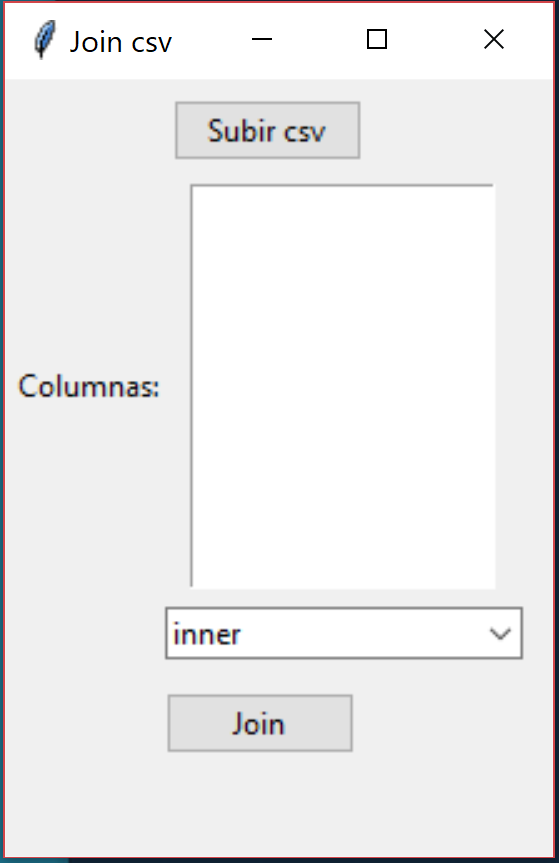
\includegraphics[width=0.7\textwidth]{manual/join-inicial}
	\caption{Aplicación de escritorio para juntar ficheros CSV}
	\label{fig:manual/join-inicial}
\end{figure}
\FloatBarrier

Una vez iniciada, habrá que pulsar el botón `Subir csv' y seleccionar todos los ficheros que quiera juntar. Otra opción es seleccionarlos de uno en uno, pulsando varias veces `Subir csv'.

Podemos usar los ficheros resultantes de exportar como CSV de nuestra aplicación (\ref{exportar}) junto con algún fichero del usuario.

Tras subir los ficheros, nos mostrará cuales son los ficheros mostrados (Figura \ref{fig:manual/join-subidos}).

\imagen{manual/join-subidos}{Selección de columnas al juntar CSV}

Si nos hemos confundido y queremos volver a empezar, pulsamos el boton `Vaciar' y volveremos al principio de la aplicación.

Se mostrará una lista de selección múltiple con las columnas comunes a todos los ficheros. Ahora tendremos que seleccionar cuáles son las columnas por las que queremos hacer join (por defecto se seleccionar `Codigo Municipio', si existe en todos los ficheros) y el tipo de join que queramos utilizar (\textit{inner}, \textit{outer}, \textit{left}, \textit{right}).

Cuando hayamos terminado, pulsamos `Join' y nos aparecerá una ventana para seleccionar la ruta donde guardar el fichero resultante.

